\section{Method}
\label{sec:graph}

%Unsupervised and graph based context aware model:

%In our model we made use of both lexical, contextual and shallow properties of the noisy text which makes use of a weighted token co-occurrence graph.

In this paper, we propose a graph based approach that models both contextual similarity features and lexical similarity features among an OOV word to be a normalized and the candidate IV words. A high level overview of our system is shown in Figure XX. An input text is first preprocessed by tokenizing and Part-Of-Speech (POS) tagging. If the text contains an OOV word, the normalization candidates are chosen by making use of the contextual features extracted from a pre-generated word-relatedness graph, as well as lexical similarity features based on edit distance, longest common subsequence ratio, and double metaphone distance. In addition, a slang dictionary is used as an external resource to enrich the normalization candidate set. The details of the approach is explained in the following sub-sections.

%%% FIGURE
\begin{figure}[htb]
\begin{center}
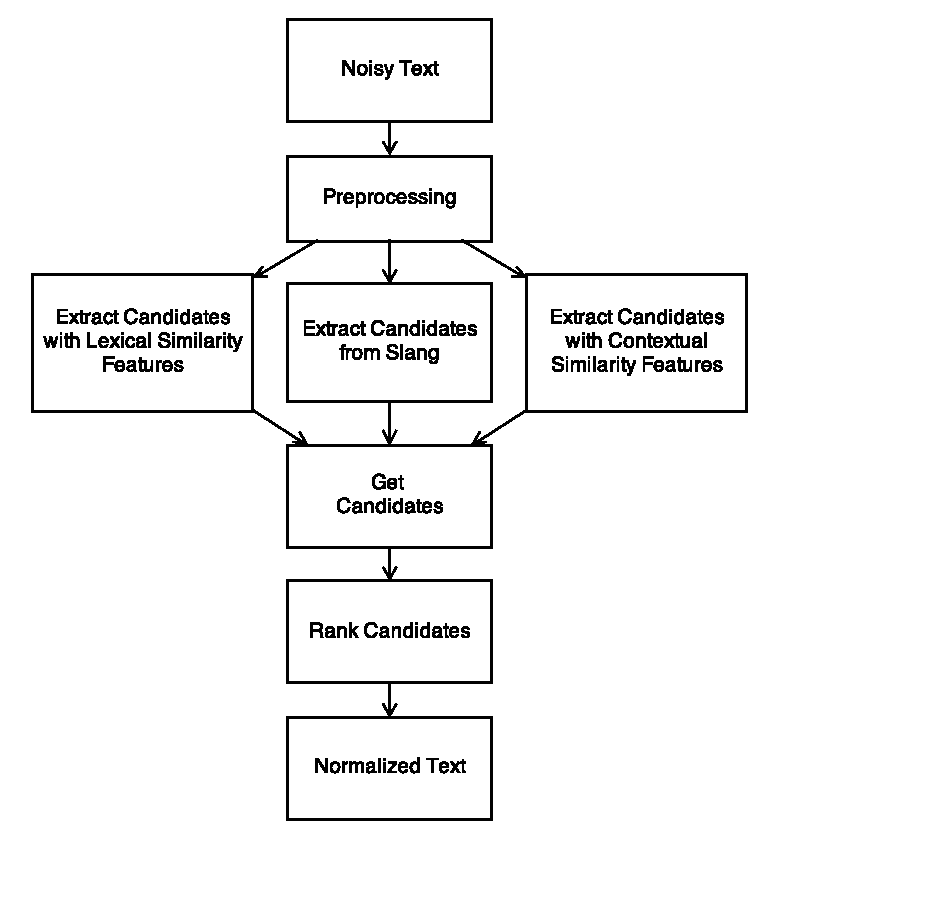
\includegraphics[scale=0.5]{overview}
\caption{This is a figure.}
\end{center}
\end{figure}

\subsection{Preprocessing}

Given a noisy token within a social media text we first tokenize and get POS tags of each token with in the text. We used CMU Ark Tweet Tagger\cite{DBLP:conf/naacl/OwoputiODGSS13}\cite{Gimpel:2011:PTT:2002736.2002747} both for tokenizing and POS tagging the tweets. Ark Tweet Tagger is a social media specific tagger and reported to perform $95\%$ accuracy over social media text. As in the table \label{tab:postags}, after preprocessing each token is given a POS tag with a confidence measure. We later make use of this confidence scores calculating the weight of an edge in our context graph.

The POS tagset of ark tagger includes some extra tags besides the standard part of speech tags that is specific to social media: Urls and emoticons; Twitter hastags \# ; twitter at-mentions (\@). One other tag that is special to social media is \~ means the token is specific to a discourse function of twitters. Lastly G stands for miscellanneous words including multiword abbreviations like

\begin{table}[!hbp]
\caption{POS tagger outputs of samples}
\label{tab:postags}
\begin{minipage}{.5\linewidth}
\begin{tabular}[h]{|llr|}
 \hline
Token & POS tag & Accuracy \\
 \hline
wit & P & 0.8793 \\
 \hline
a & D & 0.9959 \\
 \hline
beautiful & A & 0.9916 \\
 \hline
smil & G & 0.5311 \\
 \hline
\end{tabular}
\end{minipage}
\begin{minipage}{.5\linewidth}
\begin{tabular}[h]{|llr|}
 \hline
Token & POS tag & Accuracy \\
 \hline
w & P & 0.7486 \\
 \hline
a & D & 0.9920 \\
 \hline
beautiful & A & 0.9971 \\
 \hline
smile & N & 0.9712 \\
 \hline
\end{tabular}
\end{minipage}
\end{table}


\subsection{Graph construction}

\subsection{Graph Based Contextual Similarity}


Candidate selection from graph

\subsection{Lexical Similarity}

dictionary from graph

slang dictionary lookup

double metaphone 1
edit distance 2


longest common sub-sequence ratio



\subsection{Ranking}

butun parametetreler aynı.Hassan'ların lambdası

\begin{table}[tbhp]
\begin{centering}
\caption{Example noisy n-grams}
\label{tab:ngrams}
\begin{tabular}[h]{l}
\hline
with a beautiful smile \\
\hline
with a \textbf{beatiful} smile \\
\textbf{w} a beautiful smile \\
\textbf{wit} a beautiful \textbf{smil} \\
\textbf{wth} a \textbf{btfl} \textbf{sml} \\
\textbf{w} a \textbf{btfl smle} \\
\hline
\end{tabular}
\par\end{centering}
\end{table}





We tried to overcome this by building a distance aware co-occurrence representation of an n-gram language model. We builded a  graph, nodes representing the tokens and edges representing the co-occurrence relation between tokens.

Each node includes a token and tokens' POS tag.

A node consists of four properties \textit{id, ovv, freq, tag}. The token itself plus it's POS tag forms the \textit{id} field. Each token is represented with it's part of speech tag, this helps us to distinguish the different beings of tokens within the texts, helps not to propose smile as a pronoun. \textit{freq} property indicates the node's frequency count in the dataset and OOV field set to True if a token is OOV. Following Han et al. we used GNU Aspell dictionary (v0.60.6) to determine whether a word is OOV.

\begin{verbatim}
 {u'_id': u'smile|A', u'freq': 3, u'oov': False, u'tag': u'A'}
 {u'_id': u'smile|N', u'freq': 3403, u'oov': False, u'tag': u'N'}
 {u'_id': u'smile|V', u'freq': 2796, u'o0v': False, u'tag': u'V'},
\end{verbatim}

The edges graph, represents the context of tweets. It is the co-occurrence information including the distance information between words. For example the edges below would be derived from a text including the phrase ``with a beautiful smile''. The \textit{from} property indicates the first word and \textit{to} is the latter in the co-occurrence. Each co-occurrence of two words increases the weight of the representing edge with the average of their POS tag accuracy score in that specific text. If we are to expand the graph with our example phrase with the given POS tags and accuracies below. The increase in the weights would be respectively $0.9963+0.9712/2$, $0.998+0.9712/2$ and $0.9971+0.9712/2$.

\begin{verbatim}
{ "dis" : 3, "from" : "with|P", "to" : "smile|N", "weight" : 10.47095 }
{ "dis" : 1, "from" : "a|D", "to" : "smile|N", "weight" : 274.37365 }
{ "dis" : 0, "from" : "beautiful|A", "to" : "smile|N", "weight" : 240.716 }
\end{verbatim}



Our model makes use of words up to distance 4 to represent an equal form of a 5-gram language model.
